\documentclass[10pt,a4paper]{article}
\usepackage[utf8]{inputenc}
\usepackage{amsmath}
\usepackage{amsfonts}
\usepackage{amssymb}
\usepackage{graphicx}
\usepackage[utf8]{inputenc}
\usepackage[T1]{fontenc}
\usepackage{CJKutf8}
\usepackage[english,russian]{babel}
\graphicspath{{/}}
\usepackage{geometry}
\geometry{top = 2 cm}
\geometry{left = 3 cm}
\author{Будакян Ян}
\begin{document}
\begin{center}
Практическое задание по ОММ \#1, вариант 2
\end{center}
Решить задачу:
$$ \frac{\partial u}{\partial t} - u\frac{\partial u}{\partial x} = 0, \quad  -1 \leq x < 0, $$
$$u(x,0) = 2 - \frac{4}{\pi}\arctan(x+2),$$
$$u(0,t) = (2-\frac{4}{\pi}\arctan2)e^{-t}$$
Построим уравнение характеристик:
$$ \frac{dt}{1} = \frac{dx}{-u} = \frac{du}{0},$$
откуда получаем:
$$ du = 0 \rightarrow u = const,$$
$$ dt = -\frac{1}{u}dx \rightarrow t - t_0 = -\frac{1}{u}(x - x_0)$$
Подставив начальные условия, получаем уравнения для характеристик, выходящих из оси t:
\begin{equation}
x = (\frac{4}{\pi}\arctan2-2)(t-t_0)e^{-t_0},
\label{1}
\end{equation}
и оси x:
\begin{equation}
x = x_0 - t(2 - \frac{4}{\pi}\arctan(x_0+2))
\label{2}
\end{equation}
Построим графики семейства характеристик:
\begin{figure}[h]
\begin{center}
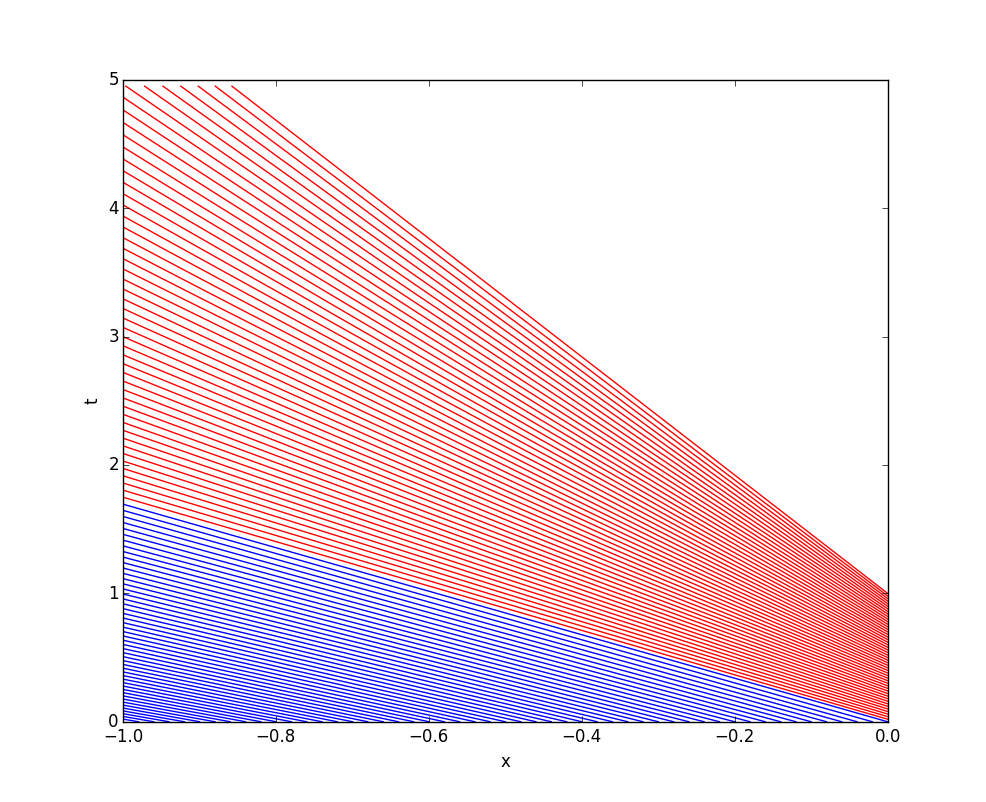
\includegraphics[scale = 0.57]{figure_1}
\caption{Семейства характеристик, красные соответствуют (\ref{1}), синие - (\ref{2})}
\end{center}
\end{figure}
\\Как видно из графика, в рассматриваемой области $ -1 \leq x < 0 $ характеристики не пересекаются.
\end{document}